
\chapter{Design Decisions}
%-------------------------------
\chapter{Implementation}
This chapter gives a detailed insights on implementation specific details of the project. In the first two sections the standalone components without ADCP related depencencies  are introduced, followd by a descrition of the parser class. The last section puts the components together and describes the architecture of the main program.  
\section{Matlab Component}
Section ... in Related Work describes the data generated by an ADCP. It was shown that the payload of each ensemble is serialized in a Matlab version 4 file format. This format is used by General Acoustics e.K. for other sensor types e.g. a sub-bottom profiler. The high possible reusability of code and algorithms related to the Matlab v.4 format predestines for a clean, independant and selfcontained code.
To ensure the the required independency the Matlab component was implemented and tested before the other components and the main program.

The implementation strongly followed the official Matlab v4. file structure documentation []. The structure defined there has a lot more possible data types and matrice types than used by the ADCP as example, in a Matlab v.4 matix the data may be stored as a sparse matrix, but is not used for ADCP ensembles. The unused features were prepared but not implemented.
% prepared code snippet
The decision to skip the implementataion of project unrelated parts helped to focus the programming efforts on other more complex parts of the project. The library is well structured and easily extendable, thus it will be a simple task to extend it if asked in forthcoming projects.
% matlab structure

The structure of the component is presented in Figure .. The \texttt{MatUtils::MatlabMatrix} is the core class of the Matlab component and stores a matlab matrix, the other classes are used to serialize and deserialize these matrices. The \texttt{MatlabMatrix} class is described in the next subsection.
\subsection{Matlab Matrix Datastructure}
This section describes the datastructure of a matlabmatrix. How it is used is described in section .. \\
As presented in figure .. a matlab matrix contains a \texttt{MatUtils::MatlabMatrixHeader}. The header contains five \texttt{uint32} Integers specifiying the rest of the Matrix and is implemented as a struct. The first integer, also called \texttt{M0PT}, is composed out of three other integers. The value is calculated as follows:
$$M\cdot1000 + 0 \cdot 100 + P\cdot 10 + T$$
M represets the Floatlayout which specifies how the float is stored in bytes. Only little and big endian were considered for this project. P is the numerical type of the matrix content and T is the matrixtype which holds if the matrix is eighter a full matrix, sparse matrix or a matrix containing text. All three values are implemented as structs their implementation is shown in figure ...

%figure impl structs
The next two integers in the header contain the number of rows and columns. Next follows a flag if the matrix has an imaginary part, which would double the amount of data used. The last integer of the Header contains the number of characters from the matrix name incremented by one to account for the string termination character.

The \texttt{MatlabMatrix} class additionaly contains a vector of \texttt{char}'s to store the matrixname.

The matrix data is stored in a templated \texttt{boost::variant} vector to allow a range of data types for the data. The fairly compicated templating (figure ..) needed to achieve this goal was taken from  a great answer at Stackoverflow [], this way the otherwise needed inheritance hierarchy was bypassed. 

\section{Sequence Buffer}
The idea of the sequence buffer has its origin at General Acoustics e.K. It serves as a Buffer between binary input streams or input queues and a consumer. The buffer has a \texttt{find()} method that searches for a sequence in the  the stream. Depending on its configuration the buffer is able to reduce read operations on the host stream
\section{Parser}
\section{ADCP Logger}
The heart of this software project was the implementation of the ADCP logger application. It integrates the seperately developed components and forms the main program. This section shows the result of the implementation, explaining the architecture and specific technical specialyties in a detailed top down approach.\\
As specified in the design decisions, the architecture is implemented in a piplined input-processing-output way. The program allows the execution of different components for each pipeline step. A configuration file is used to tell the program which component should be instantiated. The Boost Program Options library is used to parse the configuration file and set all required parameters, Figure 4.1 shows an example of a configuration file. It conveniently allows to check for invalid parameters and produces nicely formatted help output.\\
\begin{figure}[h]
\centering
      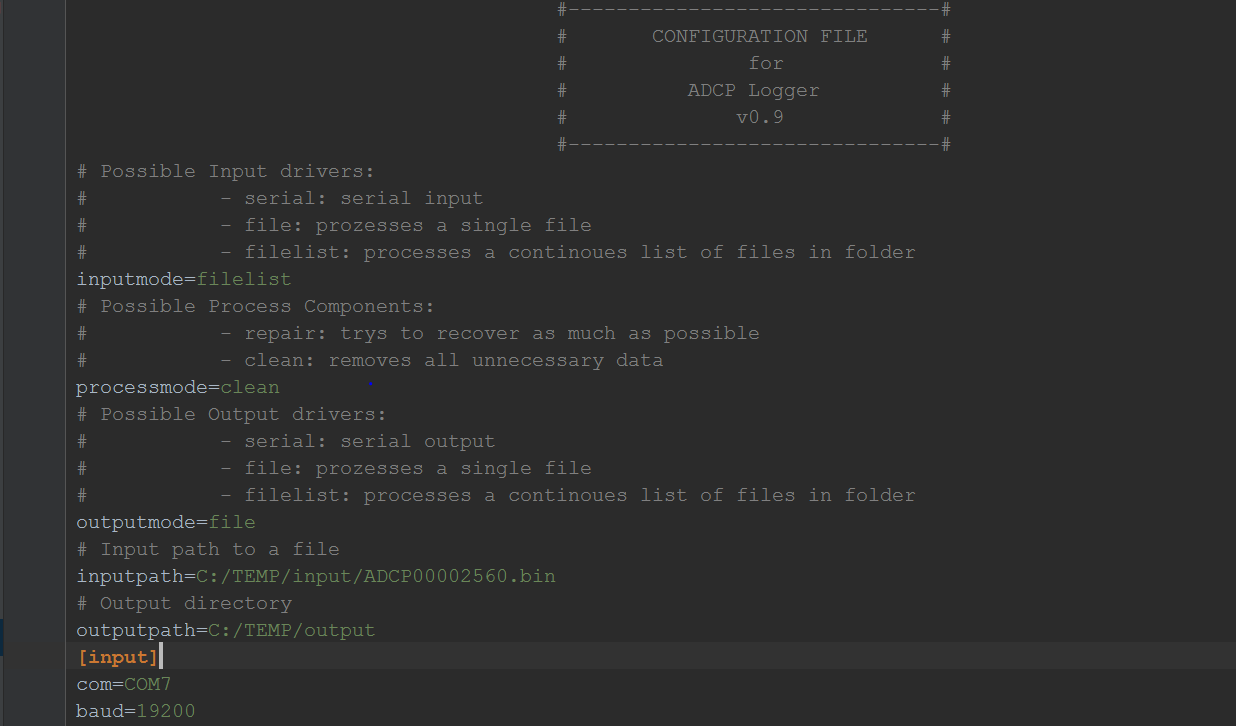
\includegraphics[width=0.7\textwidth]{config}
        \caption{A Snippet of a configuration file for the ADCP logger application}
\end{figure}

Each pipeline step is implemented as a thread. Figure 4.2 shows a dataflow model where the circles represent the threads. 
\begin{figure}[h]
\centering
      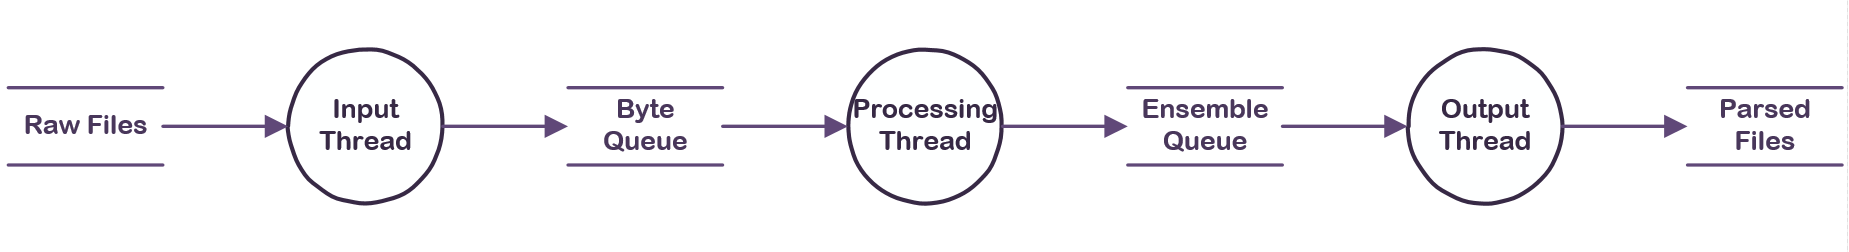
\includegraphics[width=0.95\textwidth]{dfd}
        \caption{A high-level Data-Flow-Diagram }
\end{figure}

 All threads are connected over moodycamels lockfree concurrent queues [], in the figure represented as data store objects. The queues are set up as Single-Producer-Single-Consumer (SPSC) queues and use explicit producer and consumer tokens to maximise performance. Figure 4.3 shows how the token is used to deque elements from an input queue.\\
\begin{figure}[h]	
\centering
      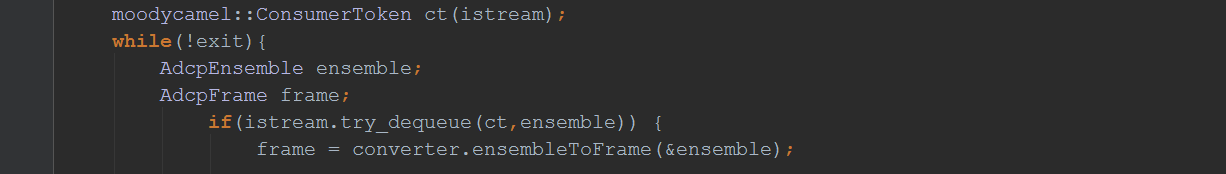
\includegraphics[width=0.95\textwidth]{ct}
        \caption{Codesnippet showing the use of consumer tokens}
\end{figure}

The threads run concurrently until the end of the execution. Each thread exits if its predecessor is finished. If this is the case, the thread synchronises with its predecessor over an atomic boolean value. A speciality here is, that the memory state of the predecessor gets propagated to the thread recieving the exit signal. In the implementation the new C++11 \texttt{std::atomic\char`_thread\char`_fence} memory barriers. This step is needed so that the thread determined to exit can reliably see if it's input queue is empty. The critical function here is the \texttt{moodycamel::size\char`_approx()} function. It returns the correct size of the queue only if the memory effects of the enqueue operations in the predecessor threads have propagated. With the use of the described memory fences this state can be reliably provided. How this was implemented is shown in figure 4.4\\
\begin{figure}[h]
\centering
      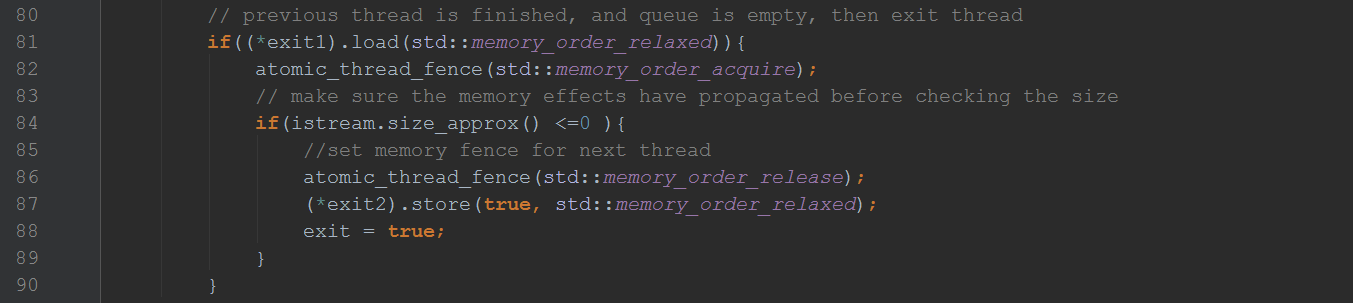
\includegraphics[width=0.95\textwidth]{memory_barrier}
        \caption{Codesnippet highlighting the memory barriers}
\end{figure}





%-------------------------------
\chapter{Testing}


 